%This research paper---as opposed to a “narrative/composition” paper (e.g., for an English course)---is a written report based on a systematic analysis that you conduct on a topic concerning Complexity Theory in the Social Sciences. Your analysis will apply a selection of concepts, theories, models, or other ideas covered in this course. The actual analysis comes first; the paper comes second, so think of this paper as a “lab report:” you write it up after you have conducted your experiment. Do not begin writing this paper before you have finished (or almost finished) your analysis, otherwise you will likely encounter serious problems. As a general guideline, papers like this are usually 15-20 pages in length. Double-space the entire paper, except the Bibliography.
%
%Use any major citation style (Turabian, MLA, Chicago); just be consistent throughout.
%
%Use any major citation style (Turabian, MLA, Chicago); just be consistent throughout.
\documentclass[pdftex,12pt]{llncs}
\usepackage[american]{babel}
\usepackage{wrapfig}
% \newcommand{\x}[1]{ }
% This is where the bibliography stuff needs to happen
\usepackage[style=apa,backend=biber]{biblatex}
\DeclareLanguageMapping{english}{american-apa}
%\addbibresource{billTolls.bib}
%\addbibresource{Projects-garbageCanCongress.bib}
\usepackage[utf8]{inputenc}
\usepackage{csquotes} % context sensitive quotes ---makes this look good
\usepackage[pdftex]{graphicx}
\usepackage{xfrac}
\usepackage{cleveref}

\begin{document}

\title{For Whom the Bill Tolls}

\subtitle{A Simulated Annealing Model of \ldots }

\author{Scott Atherley \and Clarence Dillon \and Vince Kane}

\institute{George Mason University\\
  \thanks{We wish to thank Maksim Tsvetovat who inspired this project when he introduced us to the garbage can model in his course on Computational Organizational Theory. We also wish to thank an anonymous reviewer of a previous version of this paper who inspired us rewrite it from the current perspective.}
  \email{\{satherle, cdillon2, vkane2\}@gmu.edu}}

\maketitle

%Cover page: Title, Your Name, ID, Course name, Date, and Abstract ( < 200 words).
%Title: Descriptive, well-focused, and brief. Use a subtitle to provide more information. Some hypothetical examples: “Power Law Analysis of Wealth in Ireland and Peru: A Comparative Analysis”; “Scaling in the International Airline Network“, “Governmental Capacity and Criticality in Domestic Political Instability”; “Comparing Estimates of the Pareto Exponent”. Pick a tentative title first.
%
%Do not settle on a final title until your paper is completely finished.
%

\section{Introduction}
%(approximately .5 pages) Write this section last!
%A common (bad) idea is to begin by writing this section first—it just doesn’t work because it tends to get too long and disconnected from core results. Introduce the topic of your research and its motivation. Address these questions:
%
%What is the main topic?
%
%Why is it important?
%
%What do some existing works (from readings and your own background bibliographic research) say about this topic?
%
%Conclude this section with a summary paragraph stating (one sentence each):
%the specific topic;
%main hypothesis examined in your analysis;
%approach used for this study;
%major finding. Use boldface each time you use a course term for the first time (e.g., Pareto exponent, criticality, heavy tail, exponential distribution, etc.).



\section{Methods}
%(3-4 pages) Write this section third!
%
%This section identifies and defines those concepts, models, theories, or other course ideas and tools that you used in order to carry out your analysis. Which concepts, data, theories, principles or other analytical tools from the course—from lectures or readings—did you use in this study? Which sources?
%
%Which data processing procedures? Which cases or samples? Which time periods (epochs)? Key:reproducibility! I must be able to replicate your findings, based on the information provided in this section.

\subsection{Model Overview}
In this section, we describe implementation of a model of policy formation through simulated annealing.
Conceptually, a bill is sponsored by a single legislator, reviewed and revised through two rounds of simulated annealing (first, by a network of the sponsor's friends, then by a committee of interested members), and finally voted on by the entire legislative body.
Legislators are initialized with priorities and positions on a common list of issues, with preferences stochastically generated according to quantified state priorities and party ideologies.
Legislators are connected to each other in a social network, generated using both homophily \parencite{msc01, br11} and preferential attachment \parencite{Barabasi1999}.
The initialization and simulation processes are described further in sections below.
\footnote{In the interest of brevity, we have omitted some detail descriptions of the initialization and simulation; however, these details may be found in the online supplement at \url{https://github.com/strangeintp/garbage-can-congress} and are referenced where applicable below.}

\subsection{Model Initialization}
Each model realization is initialized by generating default issue priorities and positions via the \texttt{State} object, legislators with heterogeneous priorities and positions, and a social network among the legislators.

\subsubsection{Initializing the Model Environment}
For our model, we assume that several core issues represent powerful, crystallizing factors that differentiate our simulated parties.
Thus, party "platforms" consist of vectors of positions and priorities on a set of issues that includes both \texttt{State\_Priorities} and a random sample of high-priority \texttt{Ideology\_Issues} (TBD: S?).
These vectors are used as "seeds" for the stochastic generation of individual legislator preferences.

\subsubsection{Legislator Initialization}
Each legislator's issue priorities are assigned with a stochastic preferential attachment method  (TBD: S?) to the seed values provided by the \texttt{State} object, generating a power law distribution of priorities for that legislator, and providing some correlation in legislator priorities to the extent that seed vectors are correlated through state priorities and party ideology.
We assume that party-affiliated legislators adopt the positions of their party; for all other issues (and all issues for unaffiliated legislators), positions are assigned uniform randomly from the range of allowed position values ($2^4$ for our model).

The end-result of this process is a set of legislator agents with heterogeneous but correlated policy preferences as conditioned by party ideologies and state priorities, and with the strength of correlation determined by party-alignment.

\subsubsection{Network Generation}
Model initialization is completed with a social network designed to capture the social dynamics of legislating, in that a Congressmen will naturally have a set of friends and close colleagues that he interacts with more than others. 
The network is generated using preferential attachment and total homophily over the generated preferences.
 
Preferential attachment is as described in Barabasi and Albert (1999), with $m=5$ new edges selected randomly from a \textit{pdf} of degree distribution in the sub-network of potential friends of each legislator. 
The set of potential friends is selected using an issue-priority weighted homophily over all issues (TBD: S?).

The typical outcome of this procedure is a network among legislator agents with "small-world" properties (TBD cite Watts and Strogatz), consistent with existing research on social networks in Congress \parencite{Granovetter1978}.

\subsection{Simulation Algorithm Overview}
Having defined a population of legislators and their relationship to each-other, we next establish a procedure for legislators to engage in the business of law-making.\footnote{One might argue that this is a departure from realism, as the current Congress does not appear to do this.
However, we are attempting to generalize a model of law-making in legislatures.
Some legislatures do legislate, periodically.}
In our model of law-making, the simulation sequentially repeats the following process for 200 proposals (or halts if all issues are passed into law):

\begin{enumerate}
\item Proposal:
\begin{enumerate}
\item A random legislator is chosen to sponsor a bill.
\item The sponsor proposes a draft bill on any issue that has not already been addressed by law.  This initial draft reflects the sponsor's position on that issue.
\end{enumerate}
\item Draft circulation among cosponsors:
\begin{enumerate}
\item All legislators connected to the sponsor in the social network are selected as cosponsors.
\item The cosponsors revise the draft using simulated annealing; new issues may be added to the bill during the revision process and solutions on existing issues may change (TBD: S?).
\end{enumerate}
\item Committee review:
\begin{enumerate}
\item The draft is referred to a committee, reflecting committee agenda-setting powers \parencite{cm93, cm05}.
Legislators for whom the main issue of the bill is a high priority are assigned to the relevant committee (TBD: S?).
\item The committee revises the bill by simulated annealing; again, new issues may be added and existing solutions changed.
\end{enumerate}
\item Floor vote:
\begin{enumerate}
\item The bill is referred to the floor for a vote.
\item A legislator votes `yes' to a bill when her satisfaction with it is greater than the model parameter \texttt{satisfaction\_threshold}.
\item If the bill passes by simple majority (\textgreater 50\% votes), the bill is made into law; \textit{i.e.}, the solutions addressed by the bill are recorded and the issues may not be revisited for the remainder of the realization.
\end{enumerate}
\end{enumerate}

\subsubsection{Simulated Annealing}
Bill revision is implemented by the Metropolis algorithm for simulated annealing \parencite{mrrt53, kgv}.
Our energy function is the cumulative dissatisfaction of all reviewers over all dimensions of the bill (TBD S?).  Increases of $0.1$ in dissatisfaction were accepted with probability \sfrac{1}{2} at the maximum temperature (higher satisfaction energy states are automatically accepted).
The annealing schedule is discussed in TBD: S?.

\subsection{Model Calibration}
We calibrated legislators' \textit{satisfaction thresholds}---the point at which they vote "yes" on legislation---to achieve a ~4\% pass-rate, comparable to average, historical pass-rates in the U.S. Congress (between 2\% and 7\% in recent history).\footnote{Pass rates are equal to the total number of bills passed in a given Congress divided by the total counts of introduced legislation for that Congress. Data to calculate pass rates was collected from Civic Impulse LLC (http://www.govtrack.us).\label{passfn}}

\subsection{Experiments}
Table \ref{params} identifies the model parameters and values over which a suite of experiments was run.
A factorial design was used to select combinations of values on which to run experiments.
We ran 30 realizations for each combination of values.
To keep the data set manageable, the run history for only a single realization was recorded, as a sample, for each experiment.
We recorded these metrics for each realization:  number of laws passed, number of issues addressed by law, and legislative body satisfactions over all bills before and after SA revisions.
We also calculated aggregate statistics (averages and standard deviations) and recorded the output metrics of all realizations of an experiment.

\begin{table}
 \caption{Simulation Parameter Space}
 \begin{tabular}{lp{2.25in}c}
 \hline\noalign{\smallskip}
 Parameter & Description & Value [Variation] \\
 \noalign{\smallskip}
 \hline
 \noalign{\smallskip}
 \texttt{Unaffilitated\_Fraction} & Fraction of the legislative population with no ideological party  affiliation. & [0.05, 0.5, 1.0] \\
 \texttt{Green\_Fraction} & Fraction of the party-affiliated population belonging to the \textit{Green} party. Remainder belong to the Yellow party. & [0.5, 0.75, 1.0] \\
 \texttt{Ideology\_Issues} & Ideological platform issues for the parties. & [0, 5] \\
 \texttt{State\_Priorities} & High-priority issues for all legislators. & [0, 5] \\
 \hline
 \end{tabular}
 \label{params}
\end{table}


\section{Results and Findings}
%(2 pages) Write this section first!
%
%Present your results of analysis in this section.
As described in the previous section, we experimented with variations in network structures and issue priorities to see the effects these have on productivity and satisfaction.
The fractions of party affiliation (5\%, 50\% or 100\% unaffiliated; 50\%, 75\% or 100\% of remainder in \textit{Green} party) represent a $3 x 4$ option matrix; though, with only seven real possible combinations because there are no other parties when every member is unaffiliated. 
The number of ``state-level'' priorities (0 or 5) and ``ideology'' priorities (0 or 5) represent a $2 x 2$ option matrix for each of the seven network structures, for a total of 28 possible combinations: the 28 \textit{cases}.
Throughout our research with this model, we collected metrics for the network structures, individual session history data, and aggregated case results.
This paper focuses primarily on the third set of data. 

We assessed group productivity by the number of laws that get passed (the number of \textit{pro} decisions made) in each of the 28 cases (see Figure \ref{lawspassed}). 
We examined satisfaction by the number of votes for a proposal (Figure \ref{votes}) and by how well a final draft ``fits'' individual preferences at the time of final voting (in Figure \ref{satisfaction}). 
We found that the seven network structures each produce qualitatively distinct results.
Similarly, the four priority combinations produce qualitatively distinct results. 

Most notably, 14 of the 28 cases were uniformly unproductive.
All four cases with 100\% unaffiliated bodies were completely or nearly unproductive, leaving 24 of 28 cases for further analysis.
Call these \textit{Type I} cases.
Additionally, the six remaining cases with no external priorities---\textit{Type II} cases---produced no new laws, regardless of network structure; leaving 18 viable cases.
Three more cases with a 50\% unaffiliated and 50\% \textit{Green} party make up the \textit{Type III} unproductive cases.
One other case (\#3) with 5\% unaffiliated members, 50\% \textit{Green} members and no ideology-based priorities consistently failed to produce new laws, though this case is not distinct from other that do. 

\begin{figure}[hb]
\centering
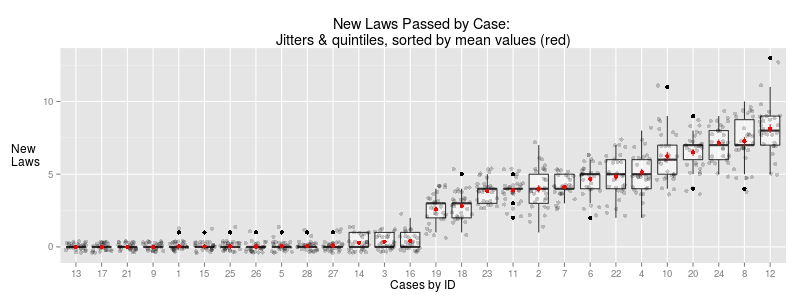
\includegraphics[width=4.9in]{laws_byJob_jitterQuints.png}
\caption[ ]{Only half of structure and priority combinations are productive. The most productive combination has 5\% unaffiliated and 95\% Green members with state and ideology priorities.} 
\label{lawspassed}
\end{figure}
 
  
The results also indicate that (average) satisfaction with final decisions decreases as more provisions are added.
Yet, adding provisions produces more votes in six of the 14 productive cases. 
This is especially true with a high number of independent members.  
This deserves further discussion and we address it in the next section.

%What did your analysis reveal?
%What did the ideas identified in the previous section show you when applied to the topic of your research?
%State your findings using vocabulary learned in the course.
%Imagine making an oral presentation of your main findings or results.
%State your first main finding or result. Then the second, and so on. You may
%want to include graphs, maps, tables, chronologies, diagrams, etc. to support your
%analysis. Label each item.

\section{Discussion}
%(3 pages including tables, figures) Write this section second!
%
%This section is entirely based on section 3.
The experiment data show discernible patters for organizational effectiveness; though, there is variation in satisfaction with decisions, support for decisions and productivity within each case.
For example, we can generalize about the importance of having external priorities for self-tasking organizations, such as the U.S. Congress, that propose decisions for group approval. 
Similarly, we see that some structures are more productive; some require more compromise; some are more satisfied with their decisions, \textit{etc}. 
In this section, we evaluate the results of the experiments to discover these rules. 
We go on to discuss some broader implications of these rules as well as some remaining questions.
Finally, we point out some implications for policy-making, organization and group dynamics. 
Figure \ref{combined} provides additional context for this section.

\begin{figure}[h]
\centering
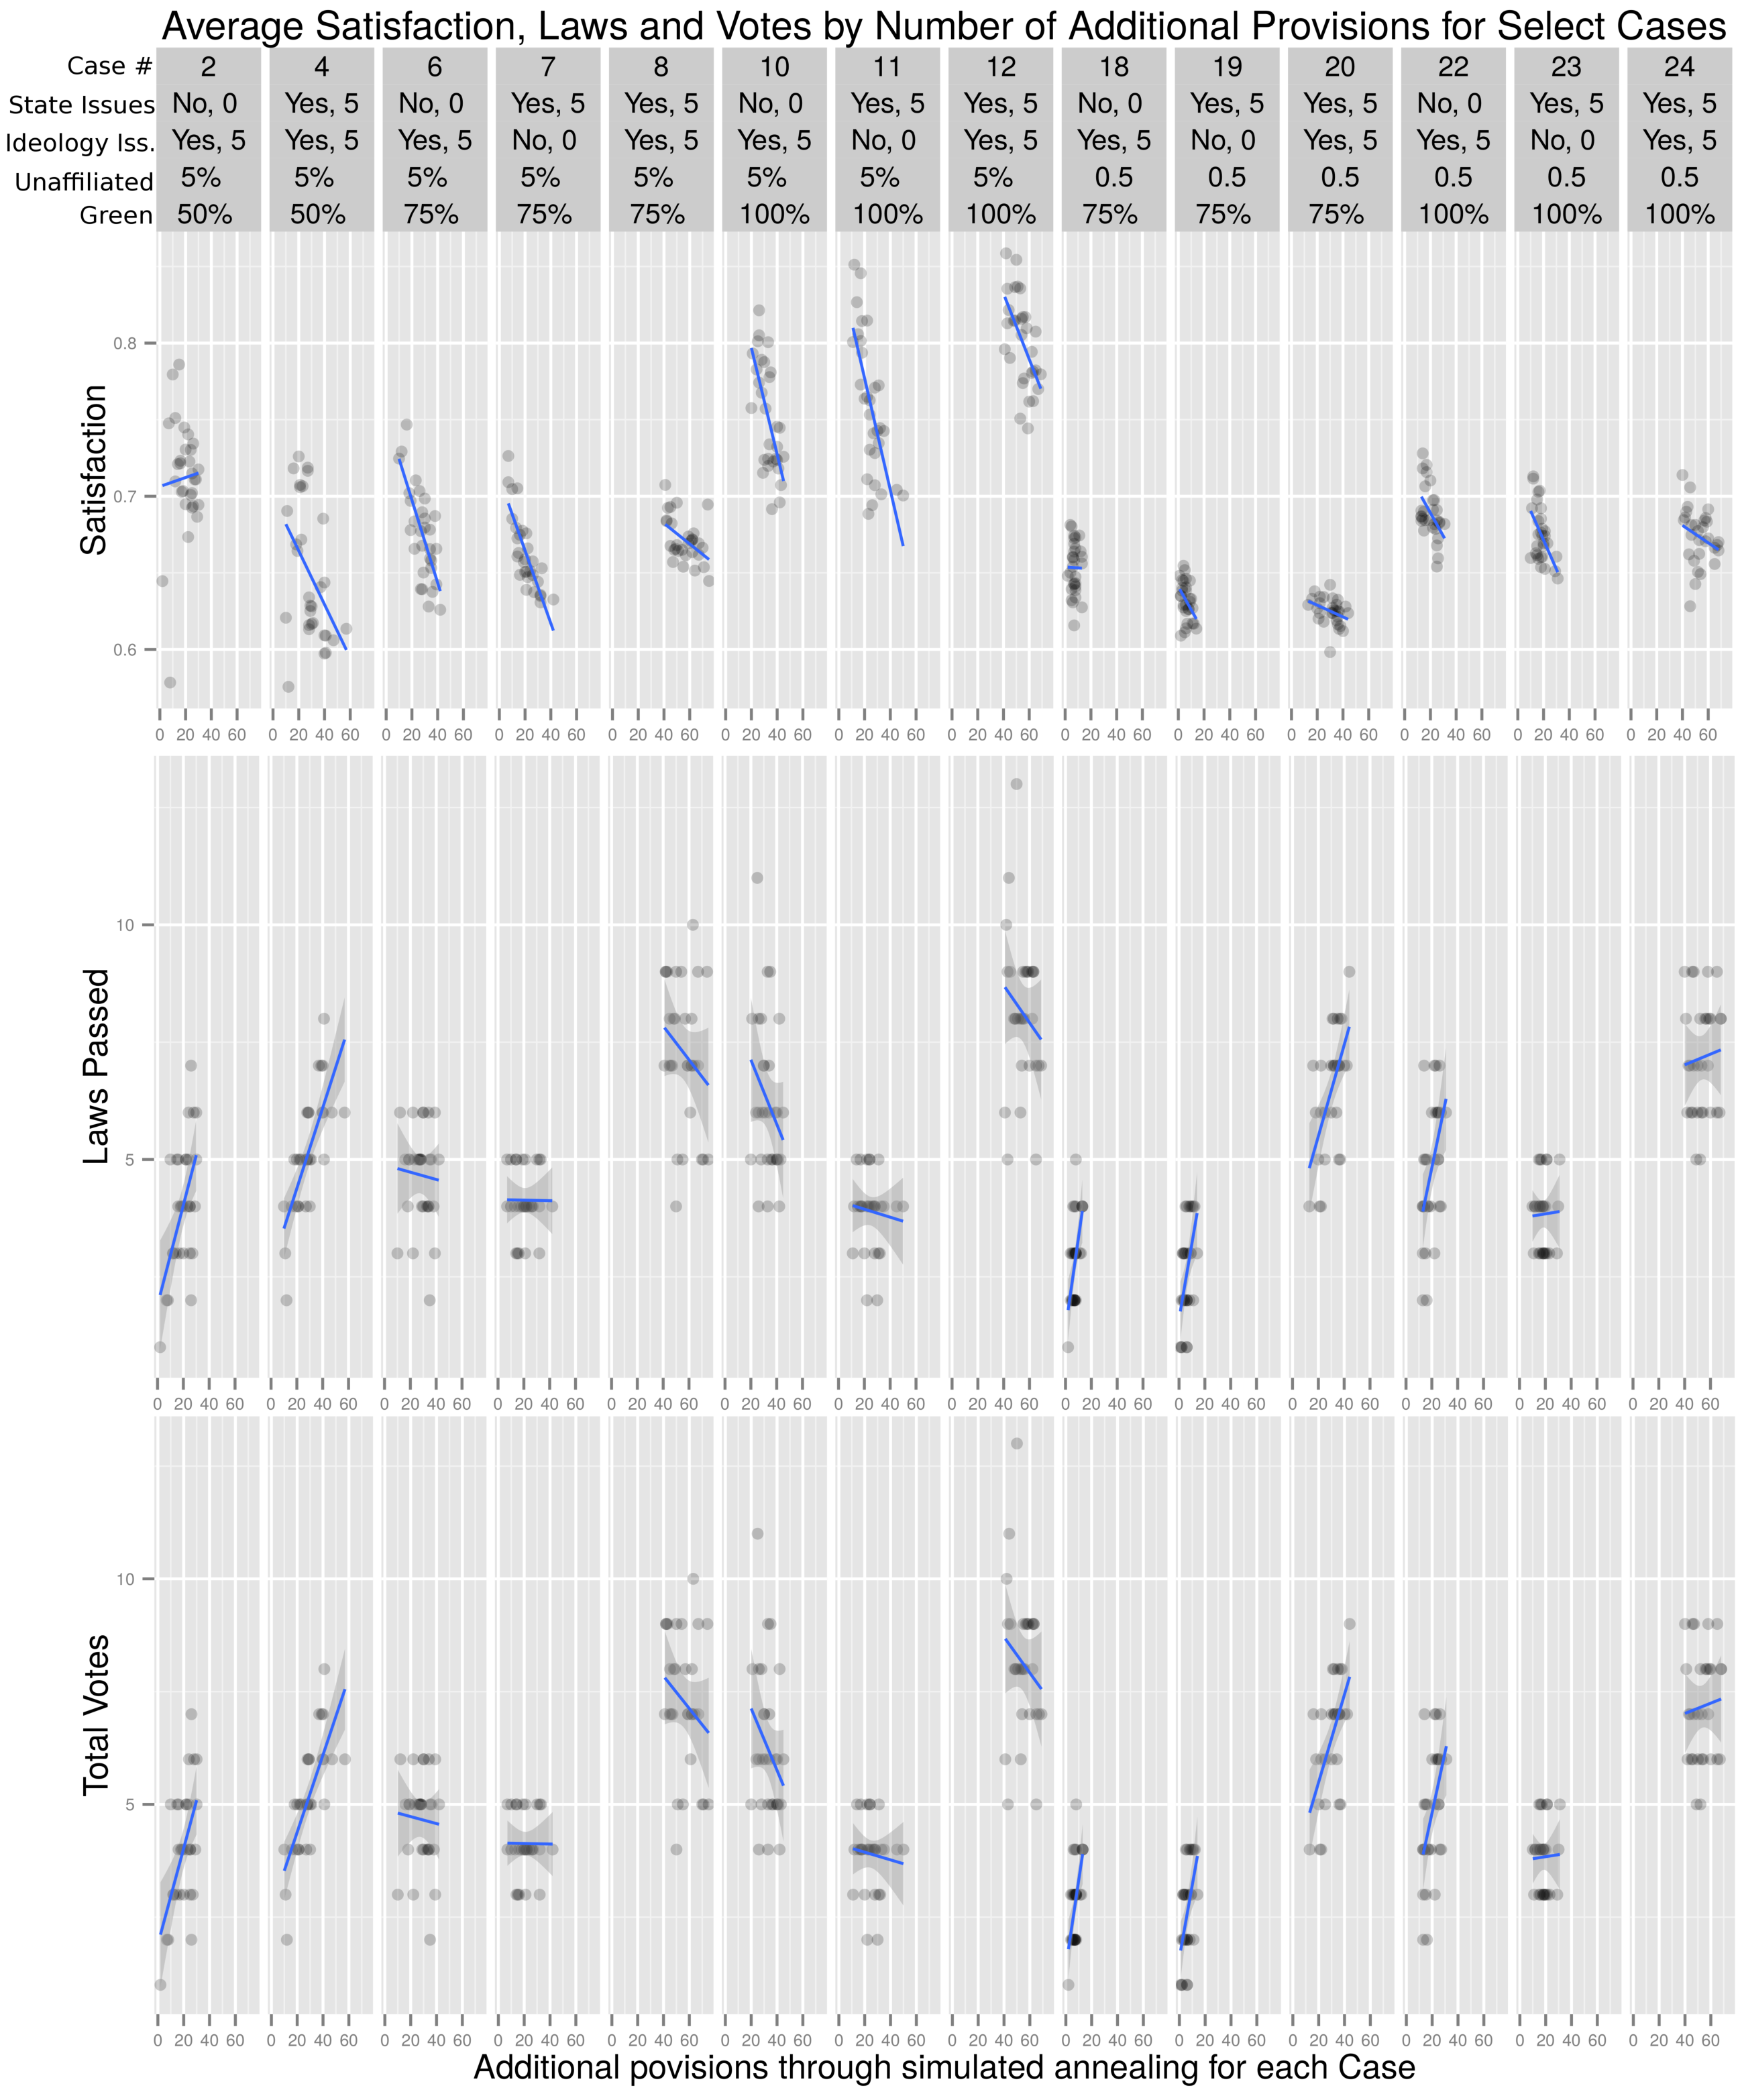
\includegraphics[width=4.25in]{combinedCases_crop.pdf}
\caption[ ]{Qualitative differences in linear fit (blue line) typify the relationship between adding provisions through simulated annealing and the average satisfaction, number of new laws and total number of votes in each case.} 
\label{combined}
\end{figure}

\subsection{Discussion of Findings}
%What do your findings mean?
%What did you learn?
%Answer the “so what?” question about your analysis.
%Provide direct answers to the question(s)/puzzle(s) in section 1 (Introduction).
%What did you expect to find before you began the study?
%What did you actually find?
%Different?
%Why?
We model Congress as a single organization, which limits applicability of the findings about our model to \textit{e.g.}, the House or the Senate; not the whole of government.
In that context, we considered the applicability of our findings to our initial motivation: we had been thinking about the U.S. Congress and the popularity of blaming recent lack of productivity on tensions between the two major political parties.  
The model results seem to not support the assertion that polarization alone leads to an unproductive legislature. 


Our cases \#1-4 typify organizational structures with 50\% of membership in the majority party---in our case, \textit{Green}---and 45\% in the opposing \textit{Yellow} party .
Consider the $2 x 2$ priority matrix for this structure: case \#1, with no external priorities is unproductive, case \#2 with only ideology priorities is productive (with wide variation), case \#3 with state priorities and without ideological priorities is unproductive and case \#4 with both state and party priorities is productive. 
However, we do not support the conclusion that the structure or the lack of ideology-based priorities that causes the current stalemate.
In eight of the 14 productive cases where 50\% of the membership falls into one of the three categories (\textit{Green}, \textit{Yellow} or unaffiliated) there is a positive correlation between the number of new laws and the number of votes as the number of additional issues get resolved with the proposed legislation.   
 
\subsection{Discussion of Broader Implications}
%Discuss the implications of your results for a broader set of ideas beyond the specific domain of analysis. Which aspects of your findings can you generalize to a larger set of patterns or cases? Interesting extentions?
It seems that self-tasking organizations are not productive without having---at least some---priorities defined externally. 
The cases with more externally-defined priorities, as a rule, are more productive than the cases with fewer externally-defined priorities. 
The cases with no externally-defined priorities were consistently unproductive.  
Organizations without any internal community (party) are similarly unproductive.

\subsection{Implications for future research}
%How would you conduct a follow-up study?
%Would you do things differently?
%How so?


\subsection{Implications for policy or other applications, if any}
%Do your findings have any implications for policy?
%Local policy?
%National domestic or foreign policy?
%Global international policy?


\section{Summary}
%(<0.5 pages)
%State the main problem or puzzle that motivated this investigation.
%State your major finding
%State your major implication
%\newpage

%\printbibliography
%BIBLIOGRAPHIC REFERENCES (1 PAGE)
%If undecided about style, follow the standard author-year format used in most social
%science publications: e.g., Smith (1990).
%
%Follow standard bibliographic reference format in this section:
%
%Last name, First Name. Year of publication. Title.

%\part{Appendices}
%Supporting documentation.
%Replication-replication-replication!
%
%Any additional supporting document (e.g., source data [BURN A CD FOR THIS], extensive tables, a treaty, Congressional hearings, etc.) or information which is too long to include in the main body of the text because it would distract or interrupt the continuity.
%
%Other guidelines:
%For text, use only 12-point Times font, as in this document. Sansserifed fonts are okay for titles or captions—do not use in text.
%
%Again, double space all text.
%Do not use single spacing.
\end{document}